\chapter{Advanced Topics}
\section{Hardware and Data Models}
\begin{sidenotebox}{The Turing Tax}
    The additional cost/overhead (performance, hardware cost, energy) of universality/general purpose computing in hardware.
    \begin{center}
        \begin{tabular}{l l p{.8\textwidth}}
                            & Example  & Description                                        \\
            General Purpose & CPU      & \textit{Jack of all trades, but a master of none.} \\
            Dedicated       & GPU, TPU & Optimised for a very specific set of operations.   \\
        \end{tabular}
    \end{center}
    The  \textit{turing tax} \& related tradeoffs of general purpose computing are discussed at length in Dr Paul Kelly's \textit{60001 - Advanced Computer Architecture} Module.
\end{sidenotebox}
\noindent
\centerline{\textit{Hardware Heterogeneity is Increasing}}
\begin{itemize}
    \item The end of moore's law the \textit{free lunch} provided decades of performance improvements by \textit{dennard scaling} is ending.
    \item Dedicated accelerators for specific applications/operations can provide increased performance by avoiding/reducing the \textit{turing tax}
    \item As a result, systems need to be able to efficiently use many different accelerators.
\end{itemize}

\begin{tcbraster}[raster columns=2,raster equal height]
    \begin{definitionbox}{GPU}
        \textit{Graphics Processing Unit}, designed for highly parallel operations on data (operating the same instructions across many threads in many warps).
    \end{definitionbox}
    \begin{definitionbox}{TPU}
        \textit{Tensor Processing Unit}, developed by Google for low precision arithmetic on tensors (matrices are 2D tensors)
    \end{definitionbox}
    \begin{definitionbox}{ASIC}
        \textit{Application-specific Integrated Circuit}. An IC designed to compute a specific application and hence with virtually no associated \textit{turing tax} overhead.
    \end{definitionbox}
    \begin{definitionbox}{Near Memory Computing}
        Accelerators built into/physically adjacent to main memory to avoid the bandwidth limitations of CPU memory access over a memory bus.
    \end{definitionbox}
\end{tcbraster}
\begin{definitionbox}{Field Programmable Gate Array (FPGA)}
    An array of programmable blocks that can be configured to a specific design (described by a developer using a \textit{hardware description language}) to perform a specific algorithm.
\end{definitionbox}
\centerline{\textit{Data Model Heterogeneity is Increasing}}
Many new data models have been developed to support specific types of application.
\begin{itemize}
    \item Key value stores used to improve performance of distributed systems through caching.
    \item Graph based models for highly interconnected data (e.g social networks) that avoid the costs associated with joins on very large relations
    \item Document based databases for flexibility \& simplicity in storing data (e.g storing BSON objects in MongoDB to support simple webapps)
\end{itemize}

\begin{tcbraster}[raster columns=2,raster equal height]
    \begin{sidenotebox}{Redis}
        \href{https://redis.io/}{Redis} is a popular in-memory key value store, often used as a cache but also usable as a key-value database.
    \end{sidenotebox}
    \begin{sidenotebox}{Memcached}
        \href{https://github.com/memcached/memcached}{Memcached} is a distributed key-value store designed for caching. Usage is nicely explained in this \href{https://github.com/memcached/memcached/wiki/TutorialCachingStory}{funny story}.
    \end{sidenotebox}
\end{tcbraster}
\begin{sidenotebox}{RedisGraph}
    A graph based database \href{https://redis.com/modules/redis-graph/}{RedisGraph} which uses adjacency matrices \& smart linear algebra to achieve a self-proclaimed title of \textit{fastest graph database}.
\end{sidenotebox}
\centerline{\textit{Workload Heterogeneity is Increasing}}
Datasets are growing larger with more kinds of workload.
\begin{center}
    \begin{tabular}{c c c c c c}
        Analytics & Transaction Processing & Inference & Data Cleaning & Data Integration \\
    \end{tabular}
\end{center}
\begin{itemize}
    \item Data integration workloads are required for the large distributed data systems
    \item Data science related workloads needed at scale (cleaning, model training and inference)
\end{itemize}

\section{CodeGen}
A typical DBMS implementation converts queries to logical, then physical plans. The kernel then invokes operator implementations specified in a query's physical plan to process the query.
\begin{center}
    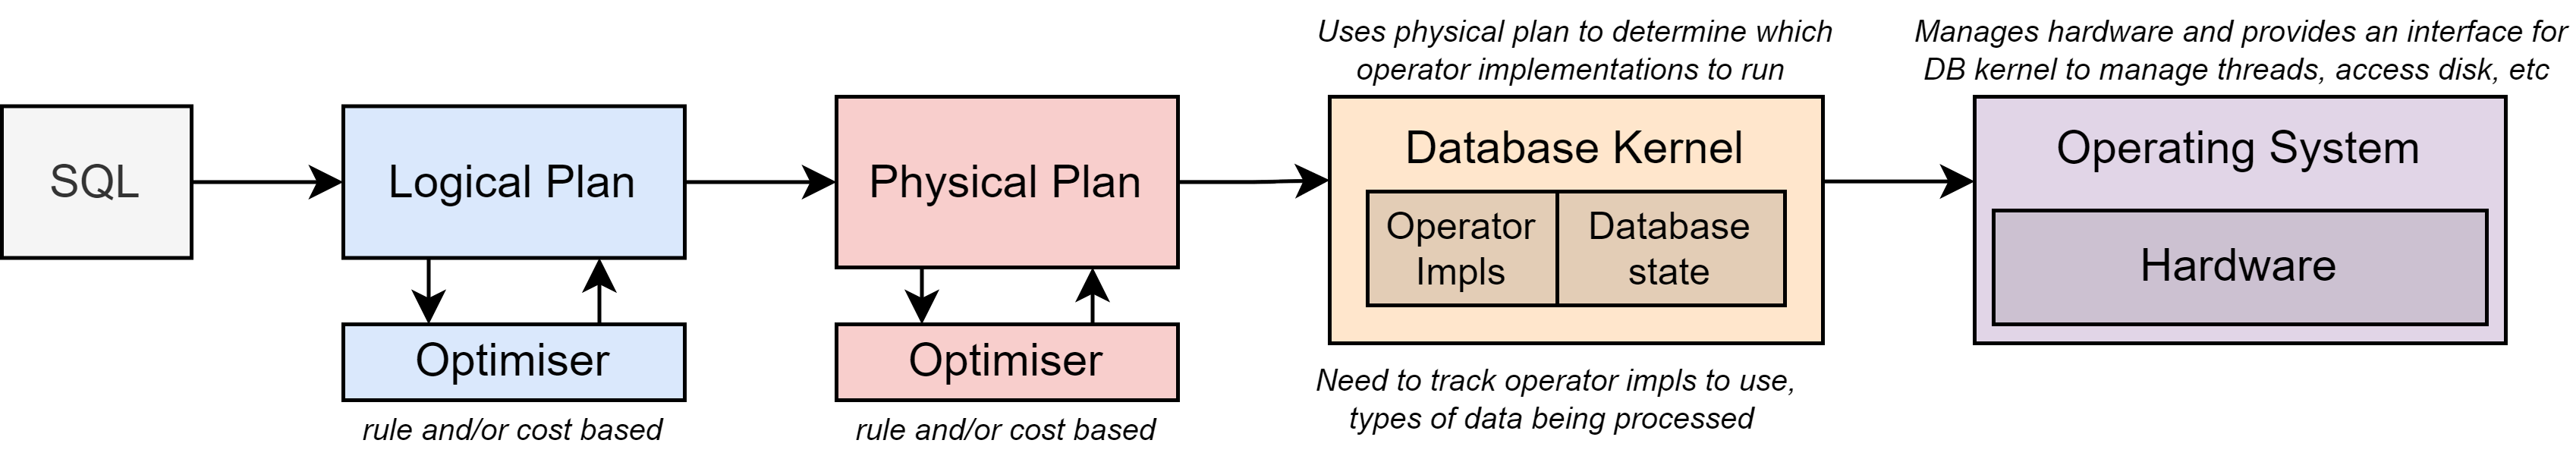
\includegraphics[width=\textwidth]{advanced_topics/images/naive_query_path.drawio.png}
\end{center}
There are several unavoidable costs/limitations to optimisation:
\begin{itemize}
    \item With volcano processing we must compose/stitch together operators at runtime, necessitating expensive virtual calls.
    \item Inter-Operator microarchitectural optimisations (e.g inlining volcano operators) are not possible as the kernel can only use operator implementations, not edit/optimise/restructure their code
\end{itemize}
Alternatively we could generate the code for operator implementations at query time, with all the information available at that time.
\begin{center}
    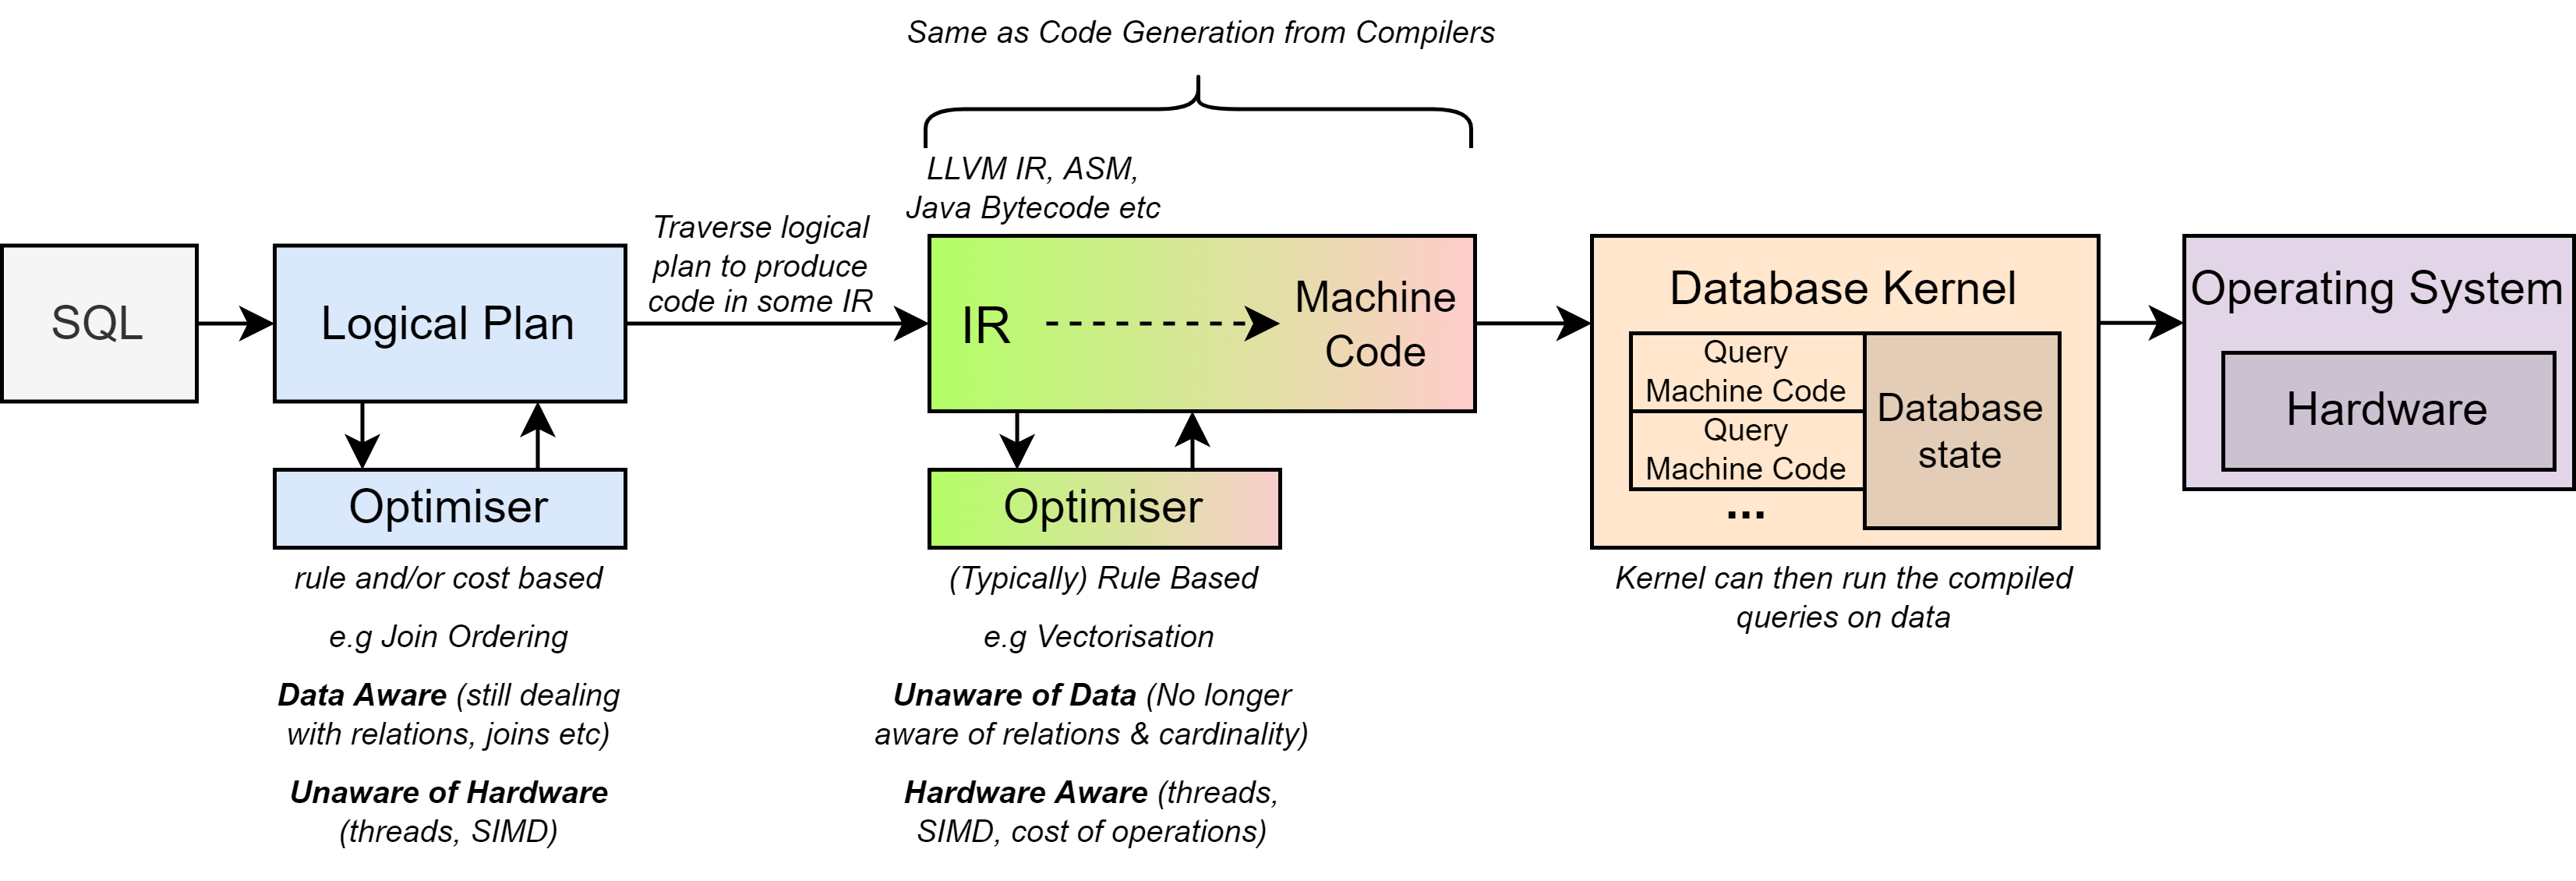
\includegraphics[width=\textwidth]{advanced_topics/images/query_compilation_path.drawio.png}
\end{center}
There are optimisations that require both data and hardware awareness, particularly relating to parallelism (needs to understand data dependencies as well as the parallelism supported by hardware).
\begin{center}
    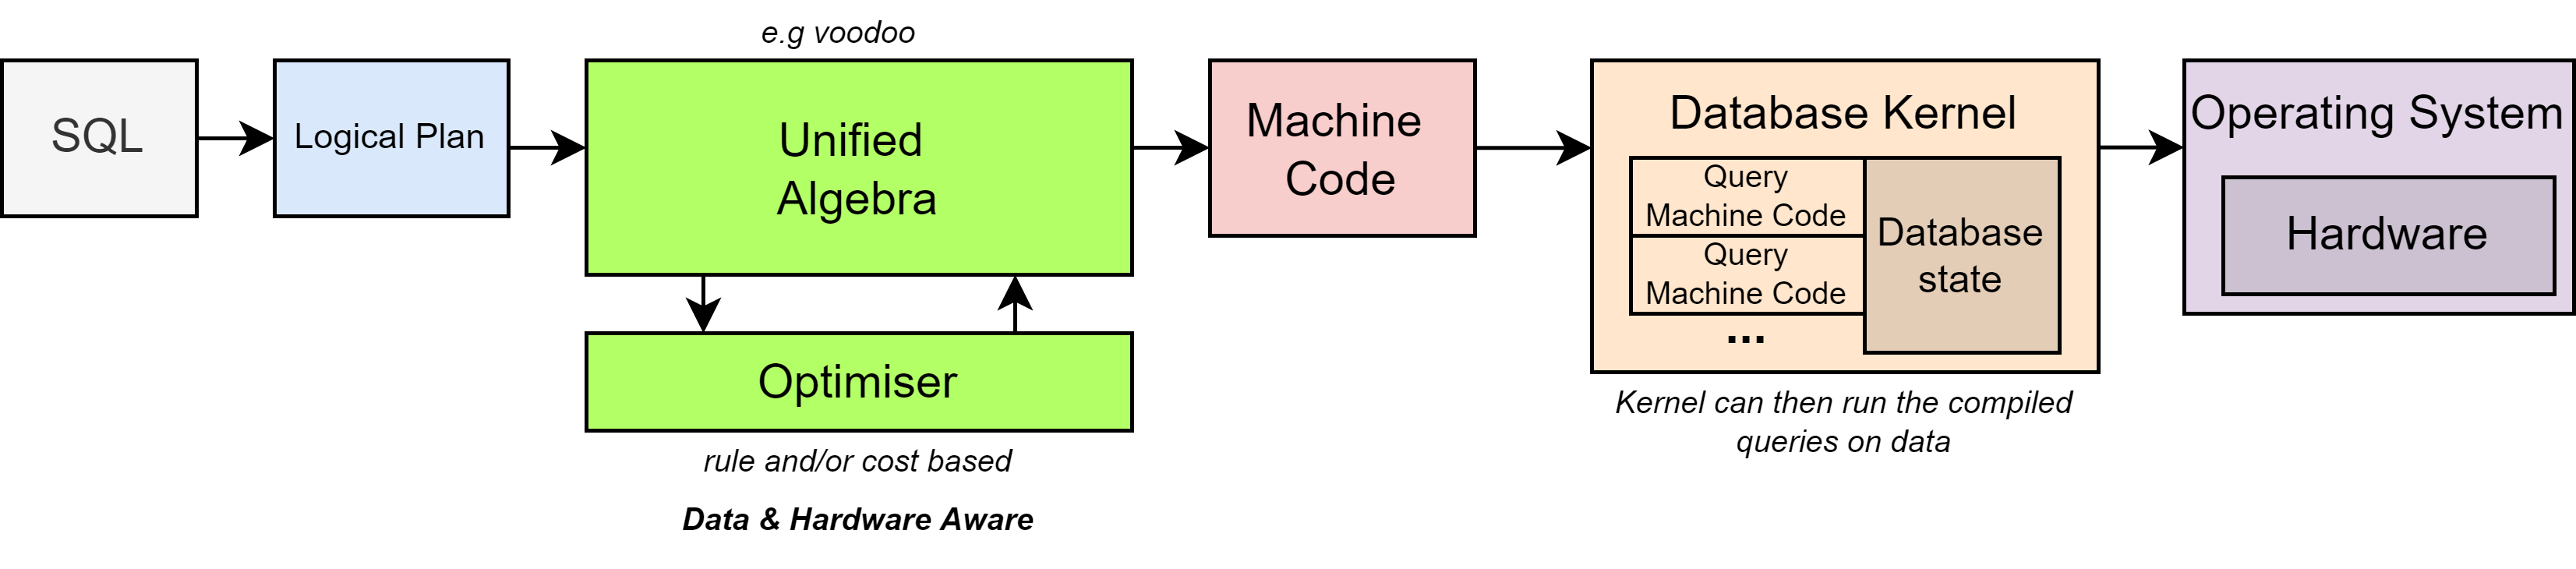
\includegraphics[width=\textwidth]{advanced_topics/images/unified_algebra_path.drawio.png}
\end{center}

\begin{definitionbox}{voodoo}
    A \textit{Vector-Dataflow Language} used as a unified algebra for code generating DBMS
    \href{https://www.cs.albany.edu/~jhh/courses/readings/pirk.pvldb16.pdf}{original paper}
\end{definitionbox}

\subsection{Vector Operations}
\[\begin{bmatrix}
        x_1, & x_2, & \dots, & x_n \\
    \end{bmatrix} + \begin{bmatrix}
        y_1, & y_2, & \dots, & y_n \\
    \end{bmatrix} = \begin{bmatrix}
        x_1 + y_1, & x_2 + y_2, & \dots, & x_n + y_n \\
    \end{bmatrix}\]
A single instruction/\textit{operation} (e.g $+$) operating on multiple data.
\begin{itemize}
    \item As each operation is independent, each can be performed in parallel.
    \item A very large vector can be partitioned and processed on multiple threads.
    \item To take advantage of this parallelism in a single thread, we can use vector extensions.
    \item Vector extensions include wider registers, and special instructions for operating on \textit{lanes} of a vector register in parallel.
\end{itemize}
\noindent For example element-wise sum over two tables (e.g previously joined in the plan).
\begin{minted}{SQL}
CREATE TABLE numbers (x BIGINT, y BIGINT); /* ... */; SELECT (x + y) as z FROM numbers;
\end{minted}
\begin{center}
    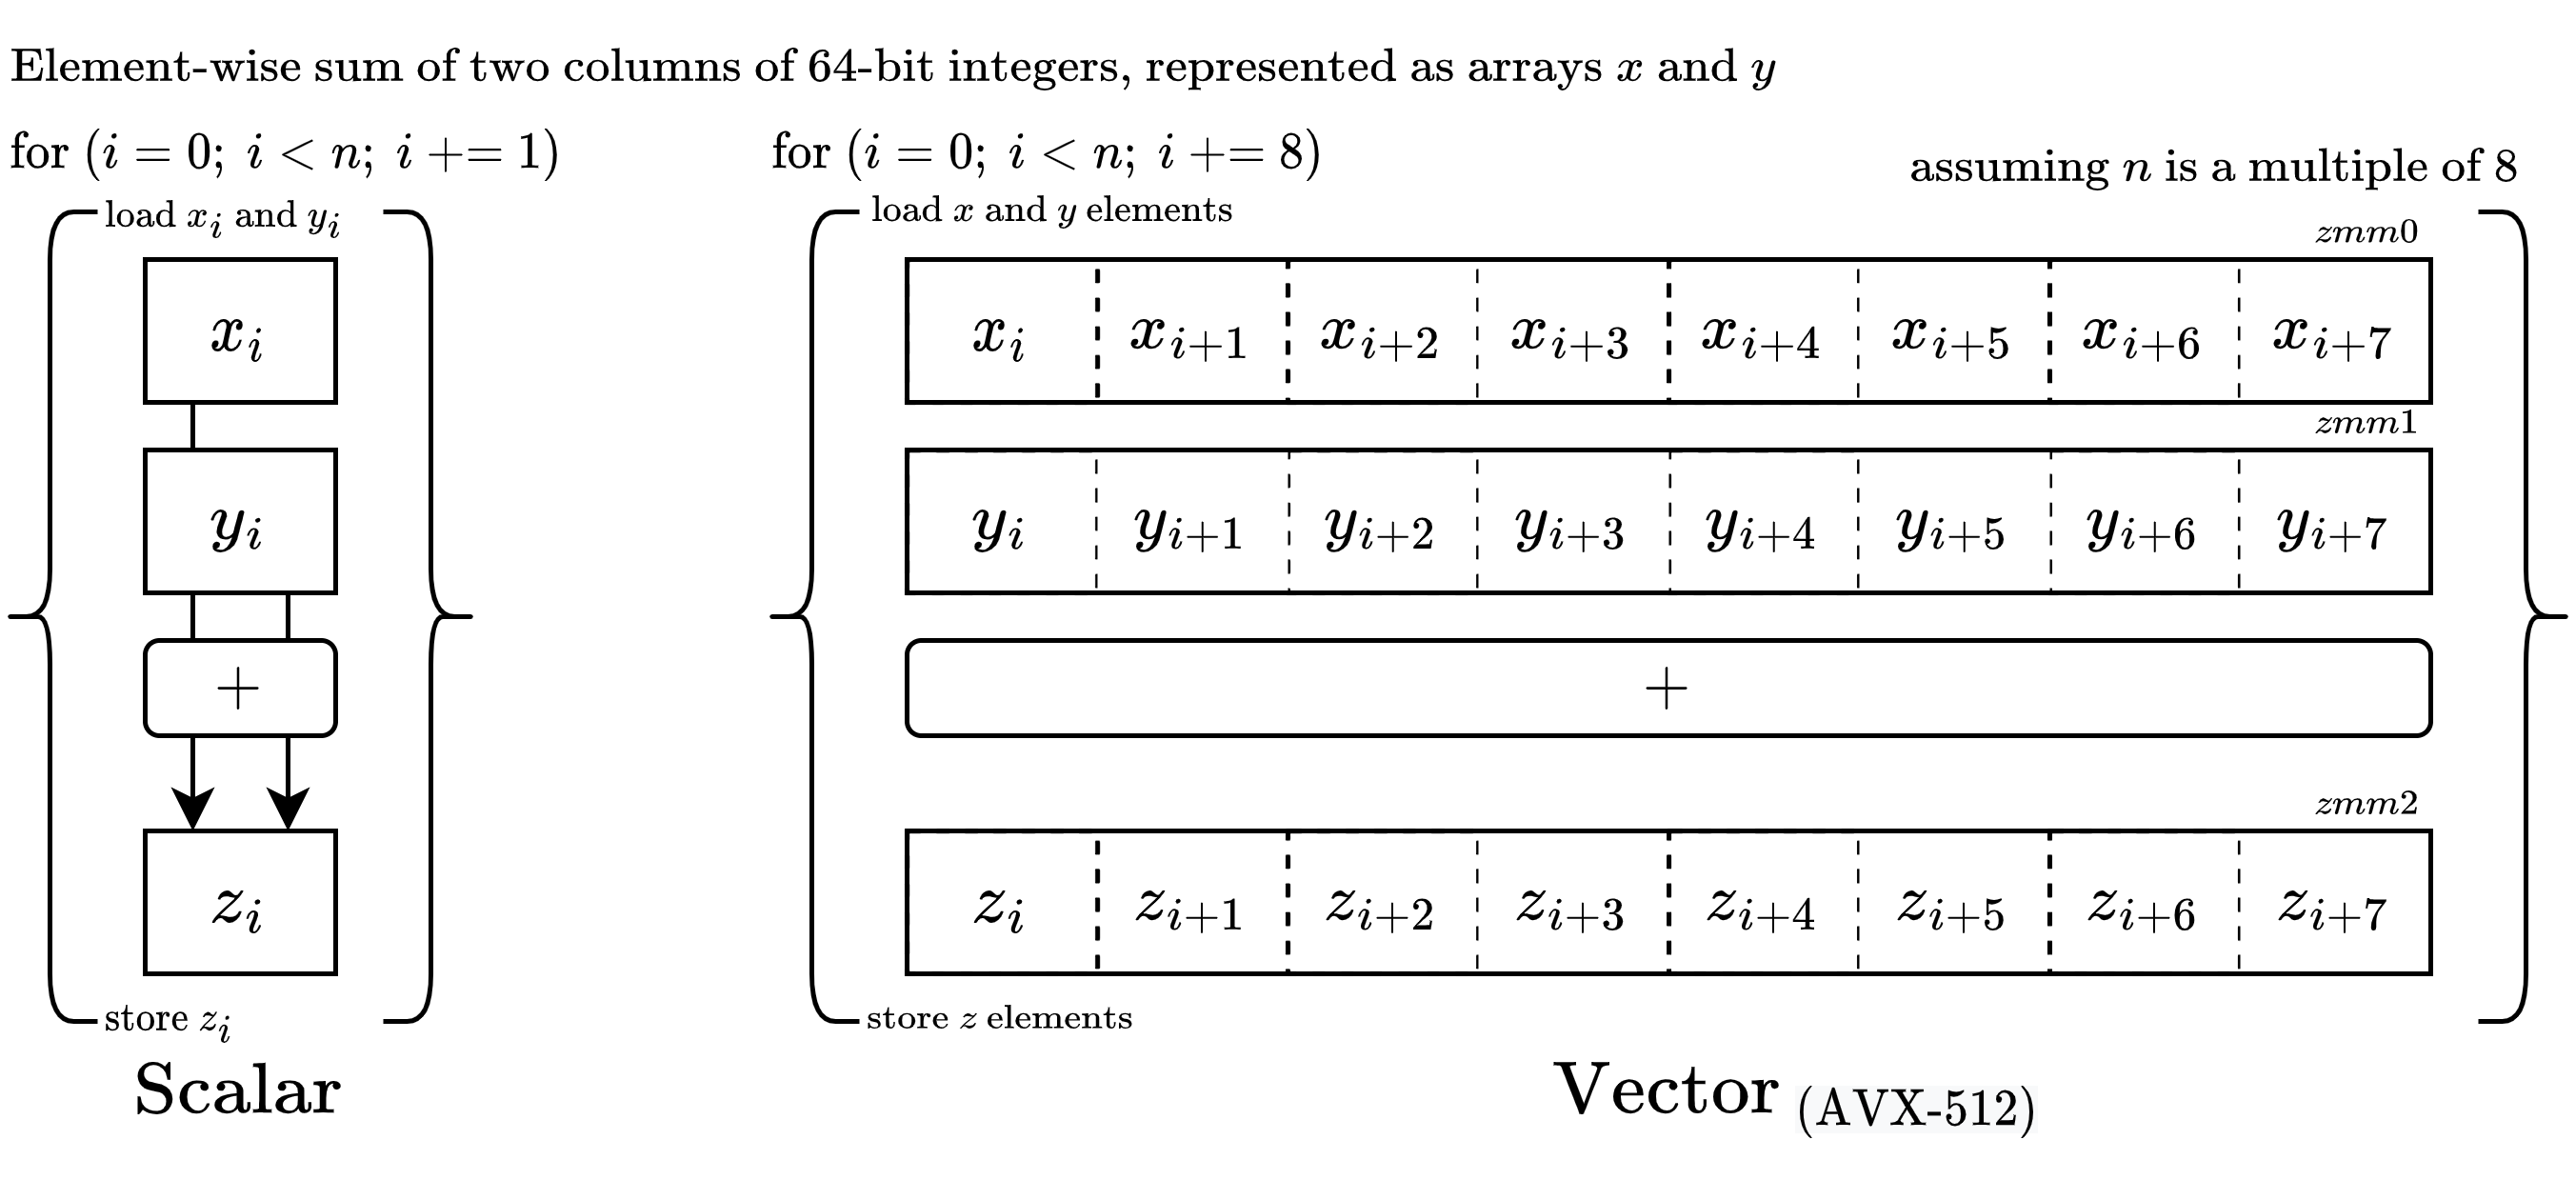
\includegraphics[width=\textwidth]{advanced_topics/images/vector_arithmetic.drawio.png}
\end{center}
Naively we could generate some \textit{scalar} code to perform the operation.
\begin{minted}{cpp}
template<size_t n>
void element_sum_scalar(int64_t x[n], int64_t y[n], int64_t z[n]) {
    for (auto i = 0; i < n; i++) z[i] = x[i] + y[i];
}
// Note: with optimisation on clang & g++ will automatically vectorize this
\end{minted}
Or we can use a vector extension we know is available on the hardware the system is running on, such as AVX-512 used here.
\begin{minted}{cpp}
#include <immintrin.h> // intel intrinsics used to ensure we use 512 bit vector instructions
#include <type_traits> // using enable_if as this code only works for n that are multiples of 8

template<size_t n>
typename std::enable_if<n % 8 == 0, void>::type 
element_sum_vec(int64_t x[n], int64_t y[n], int64_t z[n]) { 
    for (auto i = 0; i < n; i+=8) {
        __m512i xs = _mm512_loadu_si512(&x[i]);
        __m512i ys = _mm512_loadu_si512(&y[i]);
        __m512i zs = _mm512_add_epi64(xs, ys);
        _mm512_storeu_si512(&z[i], zs);
    }
}
\end{minted}
Given some call to \mintinline{cpp}{element_sum_vec<2048>(x, y, z)} we can compile:
\begin{minted}{bash}
g++ -O3 -mavx512f vectorisation.cpp  # Compiled with mavx512f to let GCC use AVX-512 instructions
\end{minted}
And extract the loop doing the summation:
\begin{minted}{nasm}
# Arrays stack allocated
.element_sum_vec:
    xor     eax, eax
.Loop:
    vmovdqu64  zmm1, ZMMWORD PTR [rsp+rax]          # xs = x[i:i+8]
    vpaddq     zmm0, zmm1, ZMMWORD PTR [r13+0+rax]  # zs = xs + y[i:i+8]
    vmovdqu64  ZMMWORD PTR [rbx+rax], zmm0          # z[i:i+8] = zs

    add rax,    64   # i += 8    * sizeof(int64_t)
    cmp rax, 16384   # i != 2048 * sizeof(int64_t)
    jne .Loop
    ret
\end{minted}

\subsection{Data Flow}
\begin{center}
    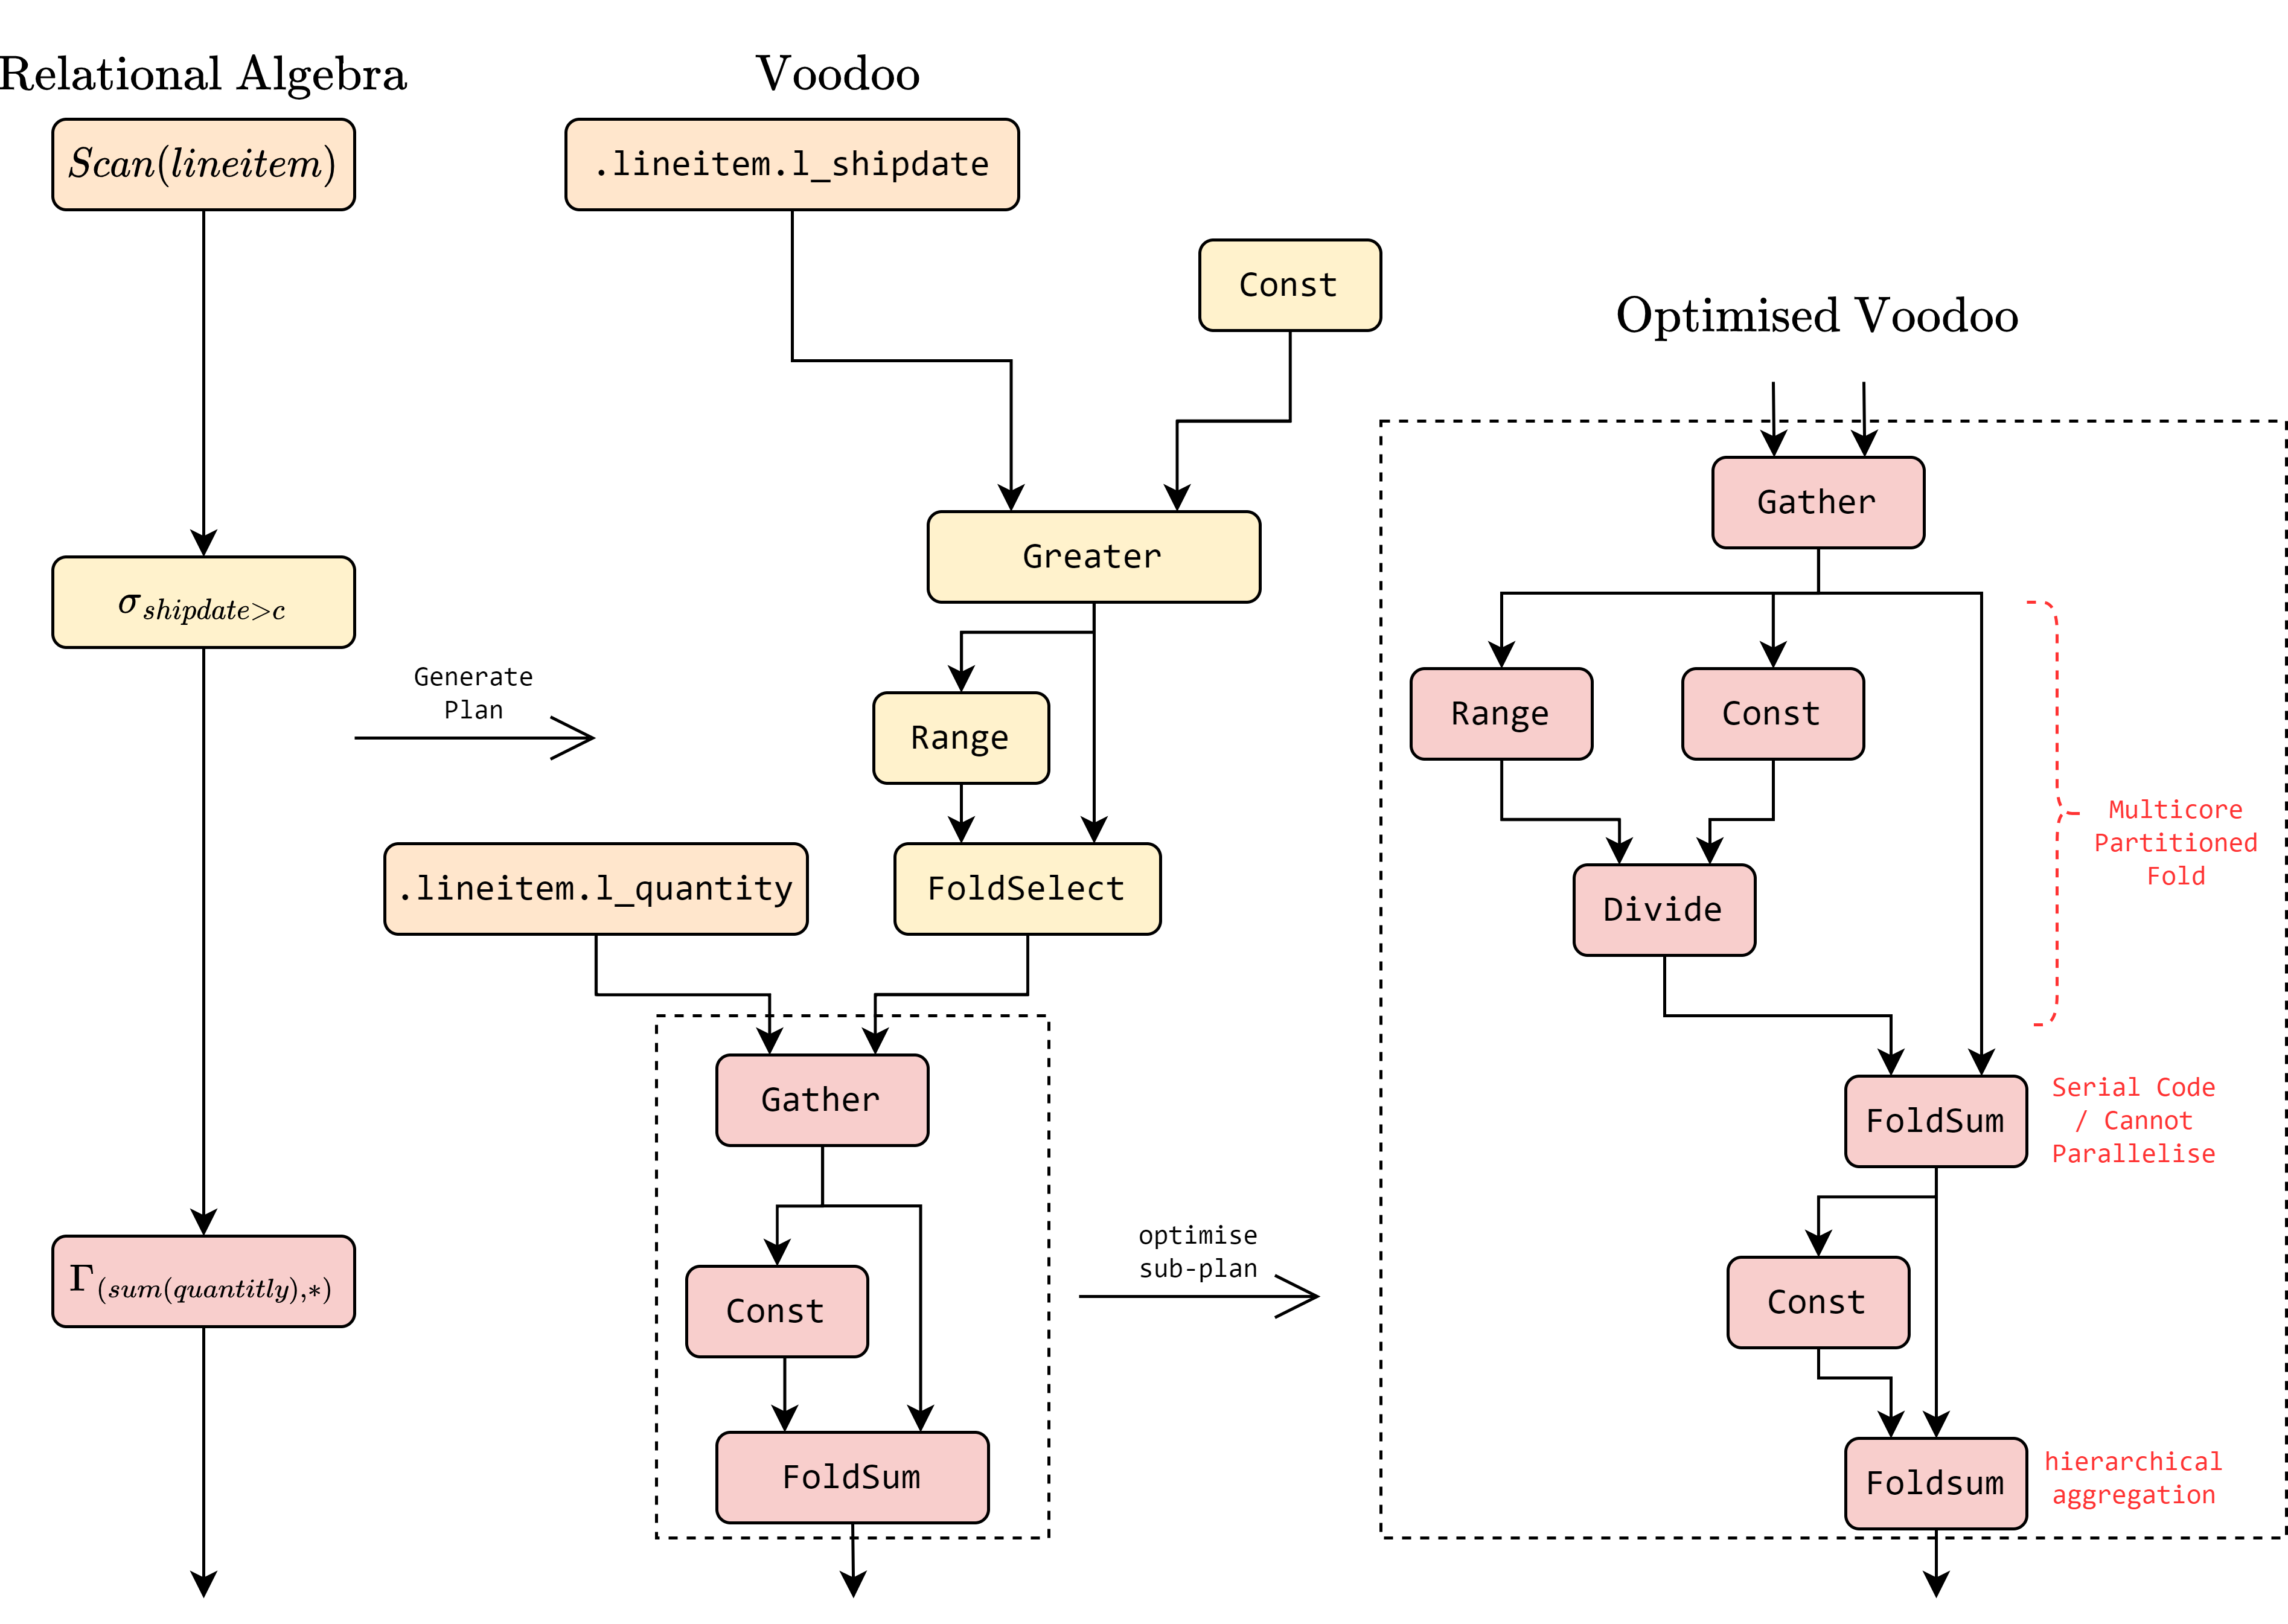
\includegraphics[width=\textwidth]{advanced_topics/images/voodoo.drawio.png}
\end{center}
\textit{Voodoo} expresses plans as a data-flow graph containing vector operations (which it can parallelise with multithreading, SIMD or GPU).

\section{Adaptive Indexing}
\subsection{Cracking}
\begin{minted}{sql}
SELECT * FROM table WHERE x BETWEEN c1 AND c2; -- Given constants c1 and c2
\end{minted}
\begin{center}
    \begin{tabular}{l p{.8\textwidth}}
        \textbf{Scan}  & \\
        \textbf{Sort}  & \\
        \textbf{Crack} & \\
    \end{tabular}
\end{center}



\subsection{Hoare Partitioning}

\subsection{Predication}
\subsection{Predicated Cracking}
\section{Stream Processing}
\section{Composable Data Processing}

